% no answer key
% \documentclass[letterpaper]{exam}

% answer key
\documentclass[letterpaper, landscape]{exam}
\usepackage{2in1, lscape} 
\printanswers{}

\usepackage{units} 
\usepackage{xfrac} 
\usepackage[fleqn]{amsmath}
\usepackage{commath}
\usepackage{cancel}
\usepackage{float}
\usepackage{mdwlist}
\usepackage{booktabs}
\usepackage{cancel}
\usepackage{polynom}
\usepackage{caption}
\usepackage{fullpage}
\usepackage{comment}
\usepackage{enumerate}
\usepackage{graphicx}
\usepackage{mathtools} 

\newcommand{\degree}{\ensuremath{^\circ}} 
\everymath{\displaystyle}

\title{Algebra Notes \\ Section 3.3 }
\author{}

\date{\today}

\begin{document}

  \maketitle

  \section{Pythagorean Theorem} % (fold)

  \begin{figure}[H]
    \centering
    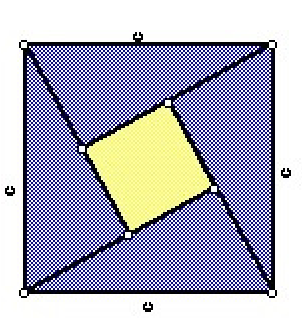
\includegraphics{proof.pdf}
    \caption{Pythagorean Theorem}
  \end{figure}
  
  The following figure was used by the Indian mathematician, Bhaskara (born 1114 CE) for another
  proof.  His proof was a little short on detail, as the entire proof was the figure and the phrase
  ``See!''.  

  The area of the big square is equal to the sum of the areas of the four triangles and the area
  of the small square.

  \begin{itemize*} 
    \item The area of each triangle is $\frac{1}{2} ab $.
    \item The area of the small square is $\del{ b - a }^2$.  
  \end{itemize*}

  \begin{align*} 
    c^2 & = 4 \del{ \frac{1}{2} ab } + \del{ b - a }^2 \\
        & = 2ab + b^2 - 2ab + a^2 \\
        & = a^2 + b^2 \\
  \end{align*}

  \section{Factoring to Product of Monomial/Binomial}

  \begin{itemize*}
    \item reverse of multiplying
    \item keep going until you can't go any farther
  \end{itemize*}

  examples:
  \begin{align*}
    12x + 8     & = 4(3x + 2) \\
    35x + 20    & = 5(7x + 4) \\
    12x^2 + 10x & = 2 \del{ 6x^2 + 5x }
  \end{align*}

  procedure:
  \begin{itemize*}
    \item factor out Greatest Common Divisor of coefficients
    \item factor out largest factor of $x$
  \end{itemize*}

  \section{Factoring by Grouping} % (fold)
  
  examples:
  \begin{align*}
    x(x - 3) + 2(x - 3) & = (x - 3)(x + 2) \\
    a(x - 1) + b(x - 1) & = (a + b)(x - 1) \\
  \end{align*}

  \section{Solving Equations} % (fold)
  \[
    ab = 0 \leftrightarrow a = 0 \text{ or } b = 0
  \]
  
  examples:
  \begin{align*}
    x^2 + 2x            & = 0 \\
    x^2                 & = -6x \\
    2x^2 + 4x           & = 0 \\
    5x^2 - 7x           & = 0 \\
    ax^2 + bx           & = 0 \\
    x(x + 1) - 2(x + 1) & = 0 \\
  \end{align*}
  
\end{document}
